%
% Capítulo 4
%
\chapter{Data Model}\label{cap:data_model}
In this chapter we'll elaborate on the various entities that compose our application and their interactions.
The complete entity relationship diagram is present in Appendix \ref{er}.

\subsection{User}

As outlined in section \ref{sec:use_cases}, our application divides users in roles, with each role being able to perform specific actions, as such, the \textbf{User} entity is a supertype, with roles being the overlapping subtypes of user, as a user can occupy multiple roles, as illustrated in Figure \ref{fig:user_entity}.

\begin{figure}[h]
	\begin{center}
		\resizebox{160mm}{!}{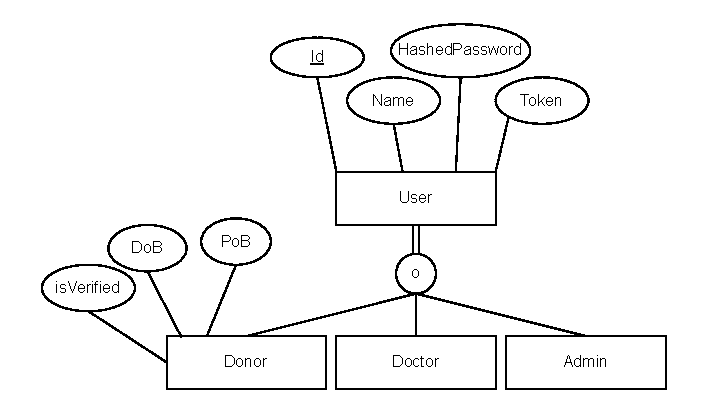
\includegraphics{./figures/User_Entity.pdf}}
	\end{center}
	\caption{User Entity.}\label{fig:user_entity}
\end{figure}

The \textbf{User} supertype contains the attributes that are common to all roles, which are as follows:

\begin{itemize}
	\item Id:A unique identifier which can be a passport or civil identification number;
	\item Name: the user's full name;
	\item HashedPassword: The user's password, stored securely as a hash, more details in section \ref{sec:security};
	\item Token: An authentication token for the user.
\end{itemize}

The \textbf{Donor} subtype contains some specific attributes, which are pertinent to this type, such as:
\begin{itemize}
	\item isVerified: boolean, indicates if donor supplied proof of identity;
	\item DoB: the donor's date of birth;
	\item PoB: the donor's place of birth;
\end{itemize}

\subsubsection{User relationships}

\begin{figure}[H]
	\begin{center}
		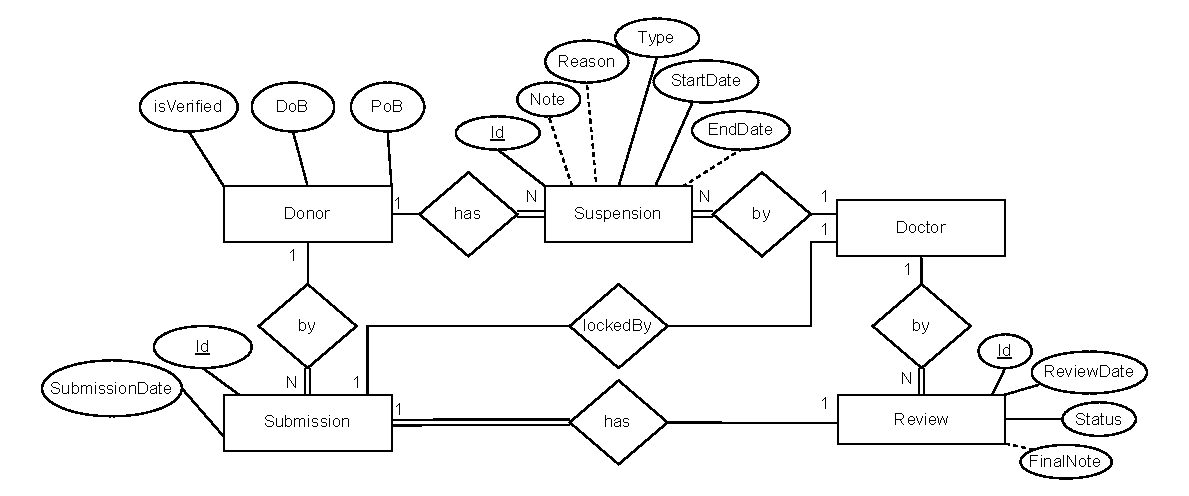
\includegraphics[width=\textwidth,height=\textheight,keepaspectratio]{./figures/User_Interactions.pdf}
	\end{center}
	\caption{User interactions.}\label{fig:user_interactions}
\end{figure}

%As mentioned before, a donor must be verified, this verification is done by an administrator upon first donation when a donor supplies proof of identity.
A \textbf{Donor} can be suspended, ie after a blood donation there's a 2 month waiting period until the next donation, this \textbf{Suspension} is created by a \textbf{Doctor}.
Each \textbf{Donor} can have multiple \textbf{suspensions}, ie multiples waiting periods after donations, and each \textbf{Doctor} can issue multiple \textbf{suspensions}.

The attributes used to characterize a \textbf{Suspension} are as follows:

\begin{itemize}
	\item \textbf{Id}:A unique identifier for the suspension;
	\item \textbf{Type}: Indicates whether the suspension is temporary or permanent;
	\item \textbf{StartDate}: The date when the suspension begins;
	\item \textbf{EndDate}: The date when the suspension ends, optional as permanent suspensions don't have an end date;
	\item \textbf{Reason}: An optional field to specify the reason for the suspension;
	\item \textbf{Note}: An optional note related to the suspension.
\end{itemize}

A \textbf{Donor} performs various pre-donation form \textbf{submissions}, which need to be reviewed by a \textbf{Doctor}, whom can \textbf{review} multiple \textbf{submissions},  with each \textbf{Submission} having a single \textbf{Review}.
The \textbf{Submission} entity's relationships are elaborated on in section \ref{sec:submission}.

A \textbf{Submission} is characterized by the date in which it was performed, \textbf{SubmissionDate}, and a unique identifier.

A review is characterize by the following attribute:
\begin{itemize}
	\item \textbf{Id}:A unique identifier for the Review;
	\item \textbf{ReviewDate}: The date in which the review was performed;
	\item \textbf{Status}: ;
	\item \textbf{FinalNote}: Optional, potential notes;
\end{itemize}





\subsection{Admin}

\begin{figure}[h]
	\begin{center}
		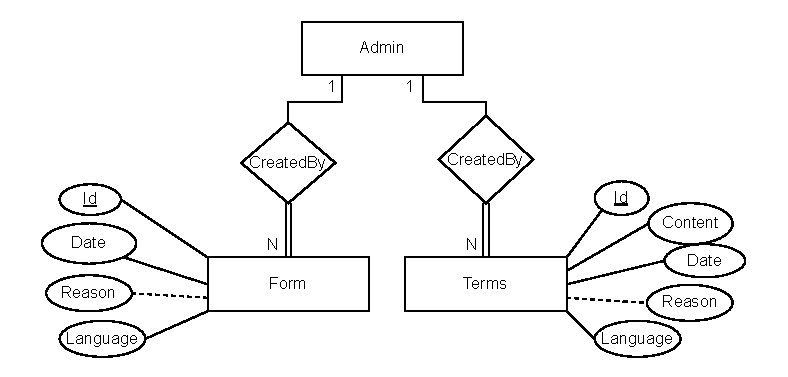
\includegraphics[width=\textwidth,height=\textheight,keepaspectratio]{./figures/Admin_Entity.pdf}
	\end{center}
	\caption{User interactions.}\label{fig:admin_entity}
\end{figure}

An \textbf{Admin} can create multiple pre-donation \textbf{forms} and multiple legal \textbf{terms} for the donation.
The \textbf{Form} entity has more relationships, but to preserve this section's scope that information is omitted but is available in section \ref{sec:form}.

The \textbf{Form} entity is characterized by the following attributes:
\begin{itemize}
	\item \textbf{Id}:A unique identifier for the form;
	\item \textbf{CreatedAt}: The date in which the form was created;
	\item \textbf{Title}: The title of the form, for ease of identification;
	\item \textbf{Language}: The language of the form stored in ISO 639-3;
	\item \textbf{isActive}: Indicates if this form is the one being presented to the donors, only one form can be active at any time for a given language;
\end{itemize}

The \textbf{Terms} entity is characterized by the following attributes:
\begin{itemize}
	\item \textbf{Id}:A unique identifier for the terms;
	\item \textbf{Content}: The actual terms;
	\item \textbf{CreatedAt}: The date in which the terms were created;
	\item \textbf{Title}: The title of the terms, for ease of identification;
	\item \textbf{Language}: The language of the terms;
	\item \textbf{isActive}: Indicates if these terms are being presented to the donors, only one of these entities can be active at any time;
\end{itemize}





\subsection{Form relationships}\label{sec:form}

\begin{figure}[h]
	\begin{center}
		\resizebox{160mm}{!}{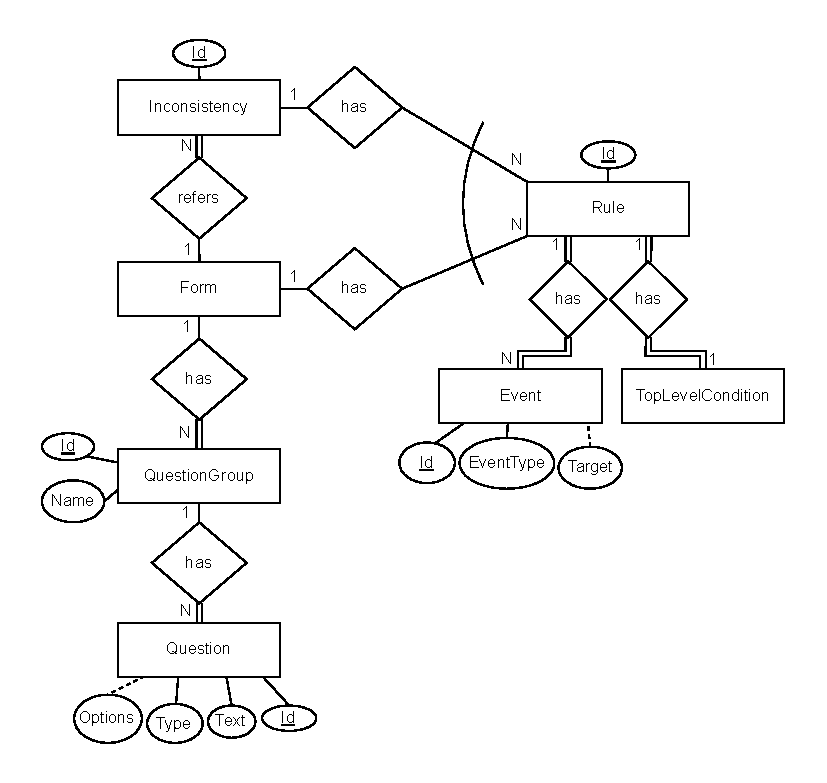
\includegraphics{./figures/Form_Entity.pdf}}
	\end{center}
	\caption{Form Entity.}\label{fig:form_entity}
\end{figure}

A \textbf{Form} is composed of a group of \textbf{questions}, this group represents a theme, and a set of \textbf{rules}, as such it has a one to many relationship with these entities.
For the sake of simplicity a rule can be defined as a logical condition, the \textbf{TopLevelCondition} entity in Figure \ref{fig:form_entity}, that triggers an event when met,ie when a donor answers that he has traveled abroad a subsequent question appears asking to which country, a further explanation of the entities that make up these conditions is presented in section \ref{sec:conditions}.

A \textbf{QuestionGroup} entity has the following attributes:
\begin{itemize}
	\item \textbf{Id}: The group's unique identifier;
	\item \textbf{Name}: The theme of the group, ie travel, health, previous donations, etc;
\end{itemize}

Logically, a \textbf{QuestionGroup} as a one to many relationship with the \textbf{Question} entity.
A \textbf{Question} entity is characterized by the following attributes:
\begin{itemize}
	\item \textbf{Id}: The question's unique identifier;
	\item \textbf{Text}: The actual question;
	\item \textbf{Type}: The type of accepted answer, ie boolean, text, multiple values, etc;
\end{itemize}

An \textbf{Event} entity is characterized by the following attributes:
\begin{itemize}
	\item \textbf{Id}: The event's unique identifier;
	\item \textbf{EventType}: The action the event performs, ie hide/show a question, allow navigation to next group, etc ;
	\item \textbf{Target}: Optional, the target of the action, ie the question to be hidden or displayed;
\end{itemize}

The \textbf{Inconsistency} entity represents a logical fallacy in sets of answers, eg a donor stating the they never traveled outside of Portugal but also stating that they've resided outside of Portugal.
This entity is compromised of a single identifying attribute,Id, and has a one to many relationship with the \textbf{Rule} entity. 


%\subsection{Inconsistency}
%
%\begin{figure}[H]
%	\begin{center}
	%		\resizebox{160mm}{!}{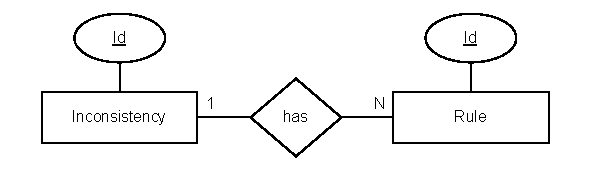
\includegraphics{./figures/Inconsistency_Entity.pdf}}
	%	\end{center}
%	\caption{Form Entity.}\label{fig:inconsistency_entity}
%\end{figure}
%
%The inconsistency entity, illustrated in Figure \ref{fig:inconsistency_entity} represents sets of answers that are illogical, ie a donor stating that they've never traveled outside of Portugal but also stating that they've resided outside of Portugal.
%This entity is compromised of a single identifying attribute,Id, and has a one to many relationship with the rule entity,mentioned in subsection \ref{sec:form}.








%\subsection{Rule}\label{sec:rule_entity}
%
%\begin{figure}[H]
%	\begin{center}
	%		\resizebox{160mm}{!}{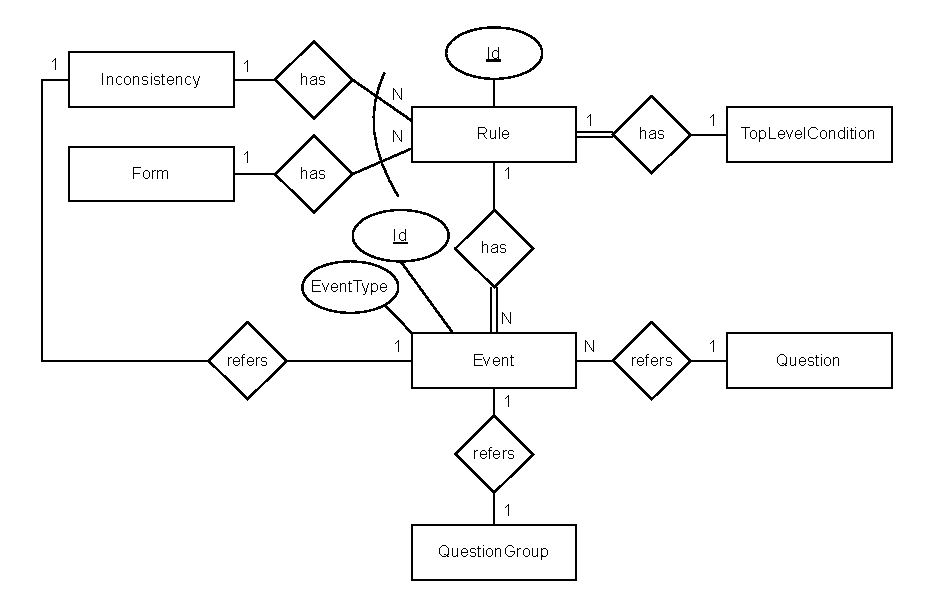
\includegraphics{./figures/Rule_Entity.pdf}}
	%	\end{center}
%	\caption{Form Entity.}\label{fig:rule_entity}
%\end{figure}
%
%The rule entity, illustrated in Figure \ref{fig:rule_entity}, has a single identifying attribute, Id, and  can be a part of a form or an inconsistency, as mentioned before.
%It has a one to one relationship with the top level condition entity, which is further elaborated in subsection \ref{conditions}, but, for now, can simply be described as the logical premises of the rule.
%
%If the logical premises are met one or more events might be triggered, hence the event entity and the rule entity have a one to many relationship.
%
%The event entity has the following attributes:
%\begin{itemize}
%	\item Id: The event's unique identifier;
%	\item EventType: The consequence of this event, ie show a question, enable the next question group, or point out inconsistent responses;
%\end{itemize}
%
%As described by the EventType attribute, and event entity can reference a question, a question group or an inconsistency.

\subsection{Conditions}\label{sec:conditions}

\begin{figure}[h]
	\begin{center}
		\resizebox{160mm}{!}{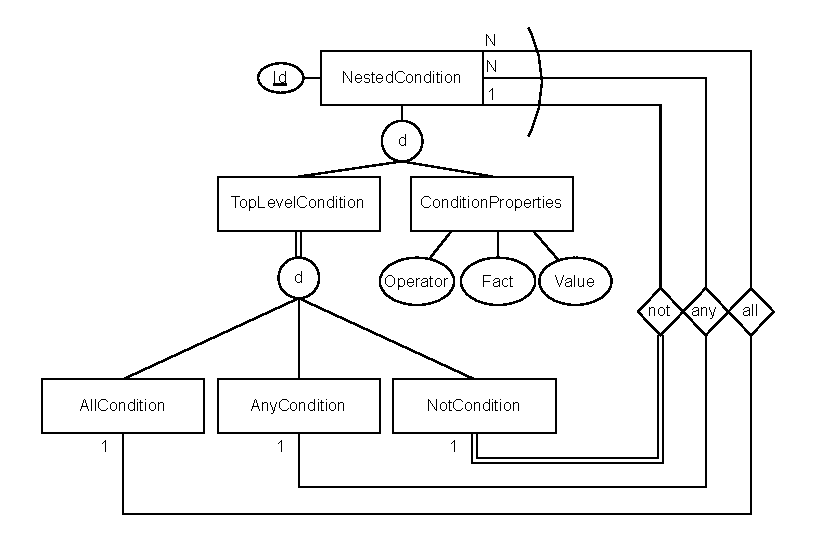
\includegraphics{./figures/Condition_Entity.pdf}}
	\end{center}
	\caption{Condition Entity.}\label{fig:condition_entity}
\end{figure}

The entities and relationships mentioned in this section reflect the types belonging to the \textbf{JSON-Rules-Engine}.
The  \textbf{NestedCondition} entity is a supertype of the \textbf{TopLevelCondition} entity and the \textbf{ConditionProperties} entity.
As the \textbf{TopLevelCondition} entity is a supertype of the \textbf{AllCondition}, \textbf{AnyCondition} a \textbf{NotCondition} entities, it can be seen as a representation of logical operators. As illustrated in Figure \ref{fig:condition_entity}, the \textbf{AllCondition} and \textbf{AnyCondition} entities have a one to many relationship with the \textbf{NestedCondition}, while the \textbf{NotCondition} as a one to one relationship, this means the \textbf{all} and \textbf{any} conditions can have multiple conditions nested inside them while the \textbf{not} condition can have a single condition nested inside it, which allows for the creation of complex boolean expressions.

The \textbf{ConditionProperties} entity represents a logical evaluation and has the following attributes:
\begin{itemize}
	\item \textbf{Operator}: The logical operator of the evaluation, ie equal, less than, greater than, etc;
	\item \textbf{Fact}: The id of the question being evaluated;
	\item \textbf{Value}: The expected value of the question being referenced.
\end{itemize}





\subsection{Submission}\label{sec:submission}

\begin{figure}[h]
	\begin{center}
		\resizebox{160mm}{!}{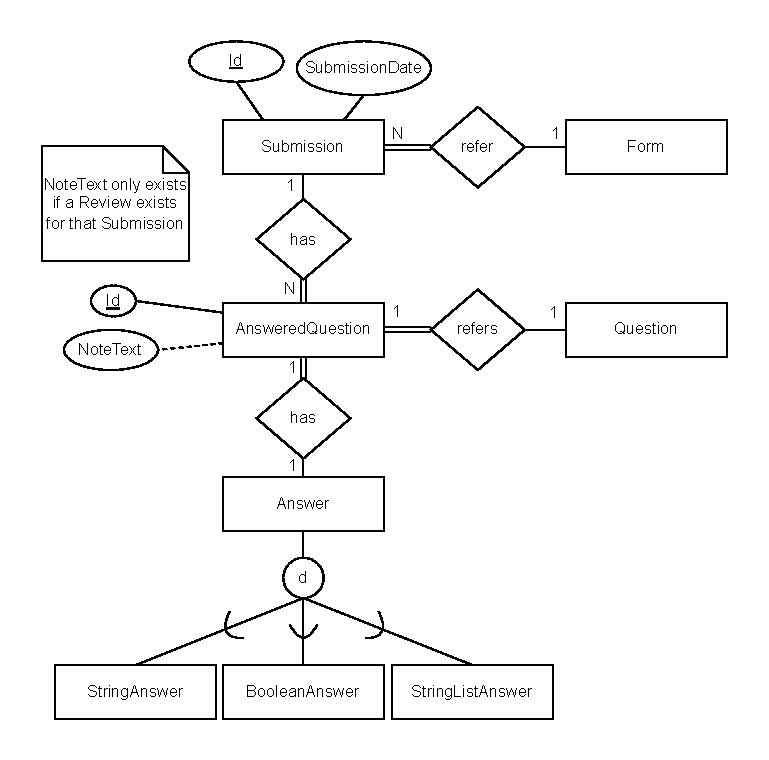
\includegraphics{./figures/Submission_Entity.pdf}}
	\end{center}
	\caption{Submission Entity.}\label{fig:submission_entity}
\end{figure}

As illustrated in Figure \ref{fig:submission_entity}, the \textbf{Submission} entity as a relationship with the \textbf{Form} entity, since a given submission pertains to a certain version of the form which changes overtime, and with the \textbf{AnsweredQuestion} entity,this entity has a \textbf{NoteText} attribute, which is optional, and represents a doctor note about the answer provided and a relationship with the \textbf{Question} entity, since every answer must refer to a question in the form.
The \textbf{AnsweredQuestion} entity also has a relationship with the \textbf{Answer} entity which is a supertype representing the possible values for the form's answers.



%\subsection{Change Log}
%
%\begin{figure}[H]
%	\begin{center}
	%		\resizebox{160mm}{!}{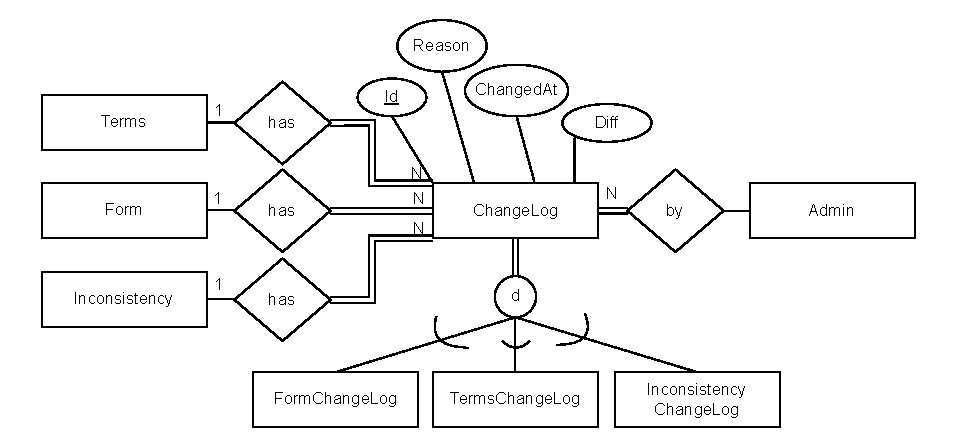
\includegraphics{./figures/ChangeLog_Entity.pdf}}
	%	\end{center}
%	\caption{ChangeLog Entity.}\label{fig:changelog_entity}
%\end{figure}
%
%To enforce admin accountability for \textbf{term}, \textbf{form} and \textbf{inconsistency} changes the \textbf{ChangeLog} entity was created and is illustrated in Figure \ref{fig:changelog_entity}.
%
%This entity has relationships with all the entities that are subjected to change and with the \textbf{Admin} entity that performed the changes.
%
%The \textbf{ChangeLog} entity serves as a supertype of the possible changes to the system, and it as the following attributes:
%\begin{itemize}
%	\item \textbf{Id}: The ChangeLog's unique identifier;
%	\item \textbf{Reason}: Optional, reason for the change;
%	\item \textbf{ChangedAt}: The date the change was performed;
%	\item \textbf{Diff}: What was changed;
%\end{itemize}

\subsection{Manual Information}

\begin{figure}[h]
	\begin{center}
		\resizebox{160mm}{!}{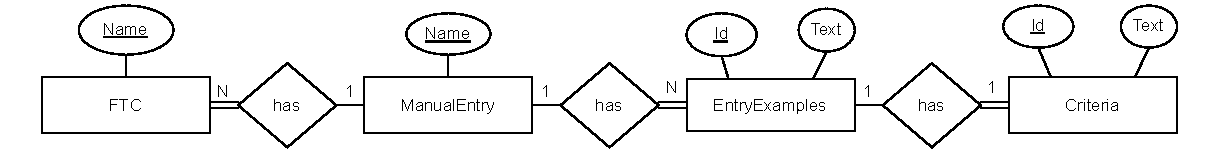
\includegraphics{./figures/Manual_Entity.pdf}}
	\end{center}
	\caption{Manual Entity.}\label{fig:manual_entity}
\end{figure}

To allow doctors to search for medication interactions with blood donations and to perform the risk vector analysis we created the \textbf{FTC} entity which is the pharmaco-therapeutic classification of the medication.
This entity has an identifying \textbf{Name} attribute, which is the name for this group of medications, e.g. analgesics and antipyretics, non steroidal anti inflammatories, etc.

The \textbf{ManualEntry} entity has an identifying \textbf{Name} attribute, which is the name used to group medications in the manual.

The \textbf{FTC} and \textbf{ManualEntry} entities have a many to one relationship as the names used in the manual might refer to more than one classification, and will possibly not have a match with any \textbf{FTC}.

The \textbf{EntryExamples} entity represents the examples presented in the manual for each entry, ie in the 2022 manual the analgesics entry contains two examples "Paracetamol, Ben U Ron, Tramadol..." and "Opioid Analgesics", so this entity has a many to one relationship with the \textbf{ManualEntry} entity and an attribute \textbf{Text}, with the examples.

Finally the \textbf{Criteria} entity which refers to whether a donor is able to donate blood or should be suspended, and whether that suspension is temporary or permanent if he's taken this medication. This entity as a one to one relationship with \textbf{EntryExamples} entity, as the evaluation of blood donation capabilities is dependent on these examples, since different medications within the same classification can lead to distinct outcomes.

\subsection{Locks}\label{sec:lock_entity}

\begin{figure}[H]
	\begin{center}
		\resizebox{160mm}{!}{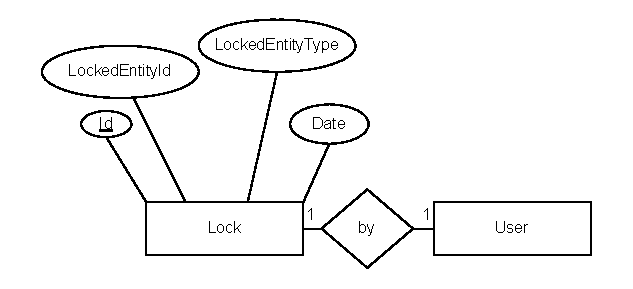
\includegraphics{./figures/Lock_Entity.pdf}}
	\end{center}
	\caption{Lock Entity.}
\end{figure}

To avoid concurrent manipulation of resources we created the \textbf{Lock} entity. This entity has a
one to one relationship with the \textbf{User} holding the lock for this resource and has the following
attributes:

\begin{itemize}
	\item \textbf{Id}: The unique identifier for this lock
	\item \textbf{LockedEntityId}: The identifier for the resource being locked;
	\item \textbf{LockedEntityType}: The type of resource being locked, i.e. submission, form, terms;
	\item \textbf{Date}: The date when the resource was locked .
\end{itemize}